% Options for packages loaded elsewhere
\PassOptionsToPackage{unicode}{hyperref}
\PassOptionsToPackage{hyphens}{url}
%
\documentclass[
]{article}
\usepackage{lmodern}
\usepackage{amssymb,amsmath}
\usepackage{ifxetex,ifluatex}
\ifnum 0\ifxetex 1\fi\ifluatex 1\fi=0 % if pdftex
  \usepackage[T1]{fontenc}
  \usepackage[utf8]{inputenc}
  \usepackage{textcomp} % provide euro and other symbols
\else % if luatex or xetex
  \usepackage{unicode-math}
  \defaultfontfeatures{Scale=MatchLowercase}
  \defaultfontfeatures[\rmfamily]{Ligatures=TeX,Scale=1}
\fi
% Use upquote if available, for straight quotes in verbatim environments
\IfFileExists{upquote.sty}{\usepackage{upquote}}{}
\IfFileExists{microtype.sty}{% use microtype if available
  \usepackage[]{microtype}
  \UseMicrotypeSet[protrusion]{basicmath} % disable protrusion for tt fonts
}{}
\makeatletter
\@ifundefined{KOMAClassName}{% if non-KOMA class
  \IfFileExists{parskip.sty}{%
    \usepackage{parskip}
  }{% else
    \setlength{\parindent}{0pt}
    \setlength{\parskip}{6pt plus 2pt minus 1pt}}
}{% if KOMA class
  \KOMAoptions{parskip=half}}
\makeatother
\usepackage{xcolor}
\IfFileExists{xurl.sty}{\usepackage{xurl}}{} % add URL line breaks if available
\IfFileExists{bookmark.sty}{\usepackage{bookmark}}{\usepackage{hyperref}}
\hypersetup{
  pdftitle={STAT 461 Midterm 1},
  pdfauthor={Xiangyu Ren},
  hidelinks,
  pdfcreator={LaTeX via pandoc}}
\urlstyle{same} % disable monospaced font for URLs
\usepackage[margin=1in]{geometry}
\usepackage{color}
\usepackage{fancyvrb}
\newcommand{\VerbBar}{|}
\newcommand{\VERB}{\Verb[commandchars=\\\{\}]}
\DefineVerbatimEnvironment{Highlighting}{Verbatim}{commandchars=\\\{\}}
% Add ',fontsize=\small' for more characters per line
\usepackage{framed}
\definecolor{shadecolor}{RGB}{248,248,248}
\newenvironment{Shaded}{\begin{snugshade}}{\end{snugshade}}
\newcommand{\AlertTok}[1]{\textcolor[rgb]{0.94,0.16,0.16}{#1}}
\newcommand{\AnnotationTok}[1]{\textcolor[rgb]{0.56,0.35,0.01}{\textbf{\textit{#1}}}}
\newcommand{\AttributeTok}[1]{\textcolor[rgb]{0.77,0.63,0.00}{#1}}
\newcommand{\BaseNTok}[1]{\textcolor[rgb]{0.00,0.00,0.81}{#1}}
\newcommand{\BuiltInTok}[1]{#1}
\newcommand{\CharTok}[1]{\textcolor[rgb]{0.31,0.60,0.02}{#1}}
\newcommand{\CommentTok}[1]{\textcolor[rgb]{0.56,0.35,0.01}{\textit{#1}}}
\newcommand{\CommentVarTok}[1]{\textcolor[rgb]{0.56,0.35,0.01}{\textbf{\textit{#1}}}}
\newcommand{\ConstantTok}[1]{\textcolor[rgb]{0.00,0.00,0.00}{#1}}
\newcommand{\ControlFlowTok}[1]{\textcolor[rgb]{0.13,0.29,0.53}{\textbf{#1}}}
\newcommand{\DataTypeTok}[1]{\textcolor[rgb]{0.13,0.29,0.53}{#1}}
\newcommand{\DecValTok}[1]{\textcolor[rgb]{0.00,0.00,0.81}{#1}}
\newcommand{\DocumentationTok}[1]{\textcolor[rgb]{0.56,0.35,0.01}{\textbf{\textit{#1}}}}
\newcommand{\ErrorTok}[1]{\textcolor[rgb]{0.64,0.00,0.00}{\textbf{#1}}}
\newcommand{\ExtensionTok}[1]{#1}
\newcommand{\FloatTok}[1]{\textcolor[rgb]{0.00,0.00,0.81}{#1}}
\newcommand{\FunctionTok}[1]{\textcolor[rgb]{0.00,0.00,0.00}{#1}}
\newcommand{\ImportTok}[1]{#1}
\newcommand{\InformationTok}[1]{\textcolor[rgb]{0.56,0.35,0.01}{\textbf{\textit{#1}}}}
\newcommand{\KeywordTok}[1]{\textcolor[rgb]{0.13,0.29,0.53}{\textbf{#1}}}
\newcommand{\NormalTok}[1]{#1}
\newcommand{\OperatorTok}[1]{\textcolor[rgb]{0.81,0.36,0.00}{\textbf{#1}}}
\newcommand{\OtherTok}[1]{\textcolor[rgb]{0.56,0.35,0.01}{#1}}
\newcommand{\PreprocessorTok}[1]{\textcolor[rgb]{0.56,0.35,0.01}{\textit{#1}}}
\newcommand{\RegionMarkerTok}[1]{#1}
\newcommand{\SpecialCharTok}[1]{\textcolor[rgb]{0.00,0.00,0.00}{#1}}
\newcommand{\SpecialStringTok}[1]{\textcolor[rgb]{0.31,0.60,0.02}{#1}}
\newcommand{\StringTok}[1]{\textcolor[rgb]{0.31,0.60,0.02}{#1}}
\newcommand{\VariableTok}[1]{\textcolor[rgb]{0.00,0.00,0.00}{#1}}
\newcommand{\VerbatimStringTok}[1]{\textcolor[rgb]{0.31,0.60,0.02}{#1}}
\newcommand{\WarningTok}[1]{\textcolor[rgb]{0.56,0.35,0.01}{\textbf{\textit{#1}}}}
\usepackage{graphicx,grffile}
\makeatletter
\def\maxwidth{\ifdim\Gin@nat@width>\linewidth\linewidth\else\Gin@nat@width\fi}
\def\maxheight{\ifdim\Gin@nat@height>\textheight\textheight\else\Gin@nat@height\fi}
\makeatother
% Scale images if necessary, so that they will not overflow the page
% margins by default, and it is still possible to overwrite the defaults
% using explicit options in \includegraphics[width, height, ...]{}
\setkeys{Gin}{width=\maxwidth,height=\maxheight,keepaspectratio}
% Set default figure placement to htbp
\makeatletter
\def\fps@figure{htbp}
\makeatother
\setlength{\emergencystretch}{3em} % prevent overfull lines
\providecommand{\tightlist}{%
  \setlength{\itemsep}{0pt}\setlength{\parskip}{0pt}}
\setcounter{secnumdepth}{-\maxdimen} % remove section numbering

\title{STAT 461 Midterm 1}
\author{Xiangyu Ren}
\date{10/12/2020}

\begin{document}
\maketitle

\hypertarget{question-3.-use-r-and-r-markdown-to-answer-the-following-questions-and-show-all-code-used-to-answer-these-questions.-assume-that-a-crd-was-used-for-an-experiment-with-three-treatments-a-b-and-c.the-following-table-records-the-response-variable-for-each-experimental-unit}{%
\paragraph{Question 3. Use R and R-markdown to answer the following
questions and show all code used to answer these questions. Assume that
a CRD was used for an experiment with three treatments (A, B, and C).The
following table records the response variable for each experimental
unit:}\label{question-3.-use-r-and-r-markdown-to-answer-the-following-questions-and-show-all-code-used-to-answer-these-questions.-assume-that-a-crd-was-used-for-an-experiment-with-three-treatments-a-b-and-c.the-following-table-records-the-response-variable-for-each-experimental-unit}}

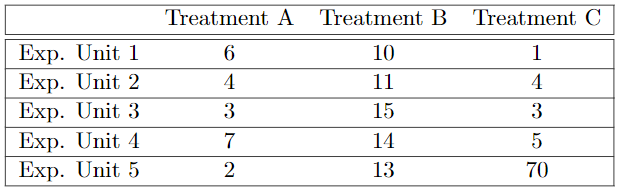
\includegraphics{table_1.png}

\hypertarget{a-create-a-box-plot-comparing-the-three-treatment-groups.-are-there-any-peculiar-points-in-the-figure}{%
\paragraph{(a) Create a box-plot comparing the three treatment groups.
Are there any peculiar points in the
figure?}\label{a-create-a-box-plot-comparing-the-three-treatment-groups.-are-there-any-peculiar-points-in-the-figure}}

\begin{Shaded}
\begin{Highlighting}[]
\NormalTok{data =}\StringTok{ }\KeywordTok{data.frame}\NormalTok{(}\StringTok{"A"}\NormalTok{ =}\StringTok{ }\KeywordTok{c}\NormalTok{(}\DecValTok{6}\NormalTok{,}\DecValTok{4}\NormalTok{,}\DecValTok{3}\NormalTok{,}\DecValTok{7}\NormalTok{,}\DecValTok{2}\NormalTok{), }\StringTok{"B"}\NormalTok{ =}\StringTok{ }\KeywordTok{c}\NormalTok{(}\DecValTok{10}\NormalTok{,}\DecValTok{11}\NormalTok{,}\DecValTok{15}\NormalTok{,}\DecValTok{14}\NormalTok{,}\DecValTok{13}\NormalTok{), }\StringTok{"C"}\NormalTok{ =}\StringTok{ }\KeywordTok{c}\NormalTok{(}\DecValTok{1}\NormalTok{,}\DecValTok{4}\NormalTok{,}\DecValTok{3}\NormalTok{,}\DecValTok{5}\NormalTok{,}\DecValTok{70}\NormalTok{))}
\NormalTok{data}
\end{Highlighting}
\end{Shaded}

\begin{verbatim}
##   A  B  C
## 1 6 10  1
## 2 4 11  4
## 3 3 15  3
## 4 7 14  5
## 5 2 13 70
\end{verbatim}

\begin{Shaded}
\begin{Highlighting}[]
\KeywordTok{boxplot}\NormalTok{(data, }\DataTypeTok{main =} \StringTok{"Comparing three treatment groups"}\NormalTok{)}
\end{Highlighting}
\end{Shaded}

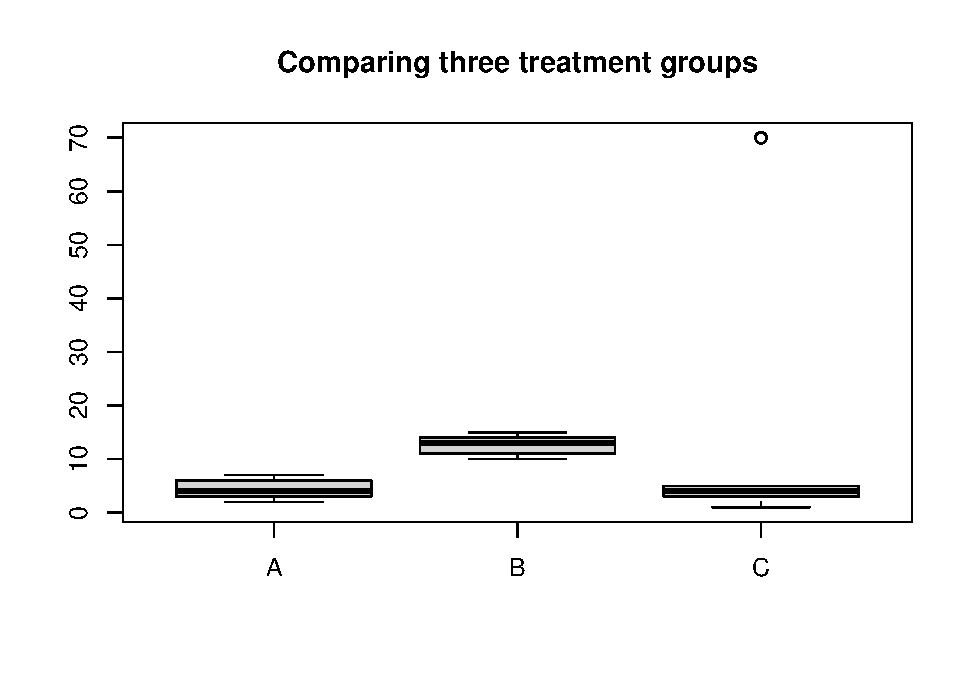
\includegraphics{Mid1_XiangyuRen_files/figure-latex/unnamed-chunk-1-1.pdf}
There is a peculiar point in group c with value 70.

\hypertarget{b-the-scientist-is-interested-in-finding-out-if-there-isanyof-the-treatments-differs-from-another.-write-down-the-appropriate-null-hypothesis-h_0-in-statistical-notation.}{%
\paragraph{\texorpdfstring{(b) The scientist is interested in finding
out if there isanyof the treatments differs from another. Write down the
appropriate null hypothesis \((H_0)\) in statistical
notation.}{(b) The scientist is interested in finding out if there isanyof the treatments differs from another. Write down the appropriate null hypothesis (H\_0) in statistical notation.}}\label{b-the-scientist-is-interested-in-finding-out-if-there-isanyof-the-treatments-differs-from-another.-write-down-the-appropriate-null-hypothesis-h_0-in-statistical-notation.}}

Null hypothesis: \[H_0:\tau_A=\tau_B=\tau_C\]

\hypertarget{c-run-a-one-way-anova-analysis-in-r-to-compute-the-p-value-for-the-hypothesis-test-outlined-in-b.-do-you-reject-or-accept-the-null-hypothesis-at-an-ux3b1.05-level}{%
\paragraph{\texorpdfstring{(c) Run a One-Way ANOVA analysis in R to
compute the p-value for the hypothesis test outlined in (b). Do you
reject or accept the null hypothesis at an \(α=.05\)
level?}{(c) Run a One-Way ANOVA analysis in R to compute the p-value for the hypothesis test outlined in (b). Do you reject or accept the null hypothesis at an α=.05 level?}}\label{c-run-a-one-way-anova-analysis-in-r-to-compute-the-p-value-for-the-hypothesis-test-outlined-in-b.-do-you-reject-or-accept-the-null-hypothesis-at-an-ux3b1.05-level}}

\begin{Shaded}
\begin{Highlighting}[]
\NormalTok{data =}\StringTok{ }\KeywordTok{data.frame}\NormalTok{(}\StringTok{"treatment"}\NormalTok{ =}\StringTok{ }\KeywordTok{c}\NormalTok{(}\KeywordTok{rep}\NormalTok{(}\StringTok{"A"}\NormalTok{, }\DecValTok{5}\NormalTok{), }\KeywordTok{rep}\NormalTok{(}\StringTok{"B"}\NormalTok{, }\DecValTok{5}\NormalTok{), }\KeywordTok{rep}\NormalTok{(}\StringTok{"C"}\NormalTok{, }\DecValTok{5}\NormalTok{)), }\StringTok{"value"}\NormalTok{ =}\StringTok{ }\KeywordTok{c}\NormalTok{(}\DecValTok{6}\NormalTok{,}\DecValTok{4}\NormalTok{,}\DecValTok{3}\NormalTok{,}\DecValTok{7}\NormalTok{,}\DecValTok{2}\NormalTok{,}\DecValTok{10}\NormalTok{,}\DecValTok{11}\NormalTok{,}\DecValTok{15}\NormalTok{,}\DecValTok{14}\NormalTok{,}\DecValTok{13}\NormalTok{,}\DecValTok{1}\NormalTok{,}\DecValTok{4}\NormalTok{,}\DecValTok{3}\NormalTok{,}\DecValTok{5}\NormalTok{,}\DecValTok{70}\NormalTok{))}
\NormalTok{model =}\StringTok{ }\KeywordTok{aov}\NormalTok{(value }\OperatorTok{~}\StringTok{ }\NormalTok{treatment, }\DataTypeTok{data =}\NormalTok{ data)}
\KeywordTok{anova}\NormalTok{(model)}
\end{Highlighting}
\end{Shaded}

\begin{verbatim}
## Analysis of Variance Table
## 
## Response: value
##           Df Sum Sq Mean Sq F value Pr(>F)
## treatment  2  386.8  193.40  0.6433 0.5428
## Residuals 12 3607.6  300.63
\end{verbatim}

According to the anova table, we can conclude that we will accept the
null hypothesis since the p-value is large than the \(\alpha\) that we
picked.

\hypertarget{d-the-scientist-now-wants-to-test-the-hypothes-is-h0fracux3c4_aux3c4_b2ux3c4_c0.-compute-the-p-value-for-this-hypothesis-test.-do-you-accept-the-null-hypothesis-at-the-ux3b1.05-level-you-must-write-out-the-test-statistic-and-the-distribution-of-the-test-statistic-for-full-credit.}{%
\paragraph{\texorpdfstring{(d) The scientist now wants to test the
hypothes is: \(H0:\frac{τ_A+τ_B}2−τ_C=0\). Compute the p-value for this
hypothesis test. Do you accept the null hypothesis at the \(α=.05\)
level? You must write out the test statistic and the distribution of the
test statistic for full
credit.}{(d) The scientist now wants to test the hypothes is: H0:\textbackslash frac\{τ\_A+τ\_B\}2−τ\_C=0. Compute the p-value for this hypothesis test. Do you accept the null hypothesis at the α=.05 level? You must write out the test statistic and the distribution of the test statistic for full credit.}}\label{d-the-scientist-now-wants-to-test-the-hypothes-is-h0fracux3c4_aux3c4_b2ux3c4_c0.-compute-the-p-value-for-this-hypothesis-test.-do-you-accept-the-null-hypothesis-at-the-ux3b1.05-level-you-must-write-out-the-test-statistic-and-the-distribution-of-the-test-statistic-for-full-credit.}}

\begin{Shaded}
\begin{Highlighting}[]
\KeywordTok{library}\NormalTok{(lsmeans)}
\end{Highlighting}
\end{Shaded}

\begin{verbatim}
## Loading required package: emmeans
\end{verbatim}

\begin{verbatim}
## The 'lsmeans' package is now basically a front end for 'emmeans'.
## Users are encouraged to switch the rest of the way.
## See help('transition') for more information, including how to
## convert old 'lsmeans' objects and scripts to work with 'emmeans'.
\end{verbatim}

\begin{Shaded}
\begin{Highlighting}[]
\NormalTok{lsm =}\StringTok{ }\KeywordTok{lsmeans}\NormalTok{(model, }\StringTok{"treatment"}\NormalTok{)}
\NormalTok{contrast1 =}\StringTok{ }\KeywordTok{c}\NormalTok{(}\DecValTok{1}\OperatorTok{/}\DecValTok{2}\NormalTok{, }\DecValTok{1}\OperatorTok{/}\DecValTok{2}\NormalTok{, }\DecValTok{-1}\NormalTok{)}
\NormalTok{contrastList =}\StringTok{ }\KeywordTok{list}\NormalTok{(}\StringTok{"1/2(tau_a+tau_b)-tau_c"}\NormalTok{ =}\StringTok{ }\NormalTok{contrast1) }
\KeywordTok{contrast}\NormalTok{(lsm, contrastList)}
\end{Highlighting}
\end{Shaded}

\begin{verbatim}
##  contrast               estimate  SE df t.ratio p.value
##  1/2(tau_a+tau_b)-tau_c     -8.1 9.5 12 -0.853  0.4104
\end{verbatim}

According to the contrast table, we can see that the estimate is -8.1
and the p-value is 0.4104. Therefore, we can conclude that we accept the
null hypothesis since 0.4104 is larger than the \(\alpha\) that we
picked. Thus \(\frac{τ_A+τ_B}2−τ_C=0\).

\hypertarget{e-while-working-on-their-analysis-the-scientist-notes-that-they-made-a-mistake-in-entering-one-of-their-data-points.-instead-y_c57.-repeat-c-but-with-this-change.-did-the-outcome-of-the-hypothesis-test-change-why-hint-compute-the-ux3c32_a-ux3c32_b-and-ux3c32_c.}{%
\paragraph{\texorpdfstring{(e) While working on their analysis, the
scientist notes that they made a mistake in entering one of their data
points. Instead, \(Y_{C,5}=7\). Repeat (c) but with this change. Did the
outcome of the hypothesis test change? Why? (Hint: Compute the
\(σ^2_A\), \(σ^2_B\), and
\(σ^2_C\)).}{(e) While working on their analysis, the scientist notes that they made a mistake in entering one of their data points. Instead, Y\_\{C,5\}=7. Repeat (c) but with this change. Did the outcome of the hypothesis test change? Why? (Hint: Compute the σ\^{}2\_A, σ\^{}2\_B, and σ\^{}2\_C).}}\label{e-while-working-on-their-analysis-the-scientist-notes-that-they-made-a-mistake-in-entering-one-of-their-data-points.-instead-y_c57.-repeat-c-but-with-this-change.-did-the-outcome-of-the-hypothesis-test-change-why-hint-compute-the-ux3c32_a-ux3c32_b-and-ux3c32_c.}}

\begin{Shaded}
\begin{Highlighting}[]
\NormalTok{data2 =}\StringTok{ }\KeywordTok{data.frame}\NormalTok{(}\StringTok{"treatment"}\NormalTok{ =}\StringTok{ }\KeywordTok{c}\NormalTok{(}\KeywordTok{rep}\NormalTok{(}\StringTok{"A"}\NormalTok{, }\DecValTok{5}\NormalTok{), }\KeywordTok{rep}\NormalTok{(}\StringTok{"B"}\NormalTok{, }\DecValTok{5}\NormalTok{), }\KeywordTok{rep}\NormalTok{(}\StringTok{"C"}\NormalTok{, }\DecValTok{5}\NormalTok{)), }\StringTok{"value"}\NormalTok{ =}\StringTok{ }\KeywordTok{c}\NormalTok{(}\DecValTok{6}\NormalTok{,}\DecValTok{4}\NormalTok{,}\DecValTok{3}\NormalTok{,}\DecValTok{7}\NormalTok{,}\DecValTok{2}\NormalTok{,}\DecValTok{10}\NormalTok{,}\DecValTok{11}\NormalTok{,}\DecValTok{15}\NormalTok{,}\DecValTok{14}\NormalTok{,}\DecValTok{13}\NormalTok{,}\DecValTok{1}\NormalTok{,}\DecValTok{4}\NormalTok{,}\DecValTok{3}\NormalTok{,}\DecValTok{5}\NormalTok{,}\DecValTok{7}\NormalTok{))}
\NormalTok{model2 =}\StringTok{ }\KeywordTok{aov}\NormalTok{(value}\OperatorTok{~}\NormalTok{treatment, }\DataTypeTok{data =}\NormalTok{ data2)}
\KeywordTok{anova}\NormalTok{(model2)}
\end{Highlighting}
\end{Shaded}

\begin{verbatim}
## Analysis of Variance Table
## 
## Response: value
##           Df Sum Sq Mean Sq F value    Pr(>F)    
## treatment  2  235.6 117.800  25.985 4.357e-05 ***
## Residuals 12   54.4   4.533                      
## ---
## Signif. codes:  0 '***' 0.001 '**' 0.01 '*' 0.05 '.' 0.1 ' ' 1
\end{verbatim}

According to the anova table, the p-value that we get is extremely
smaller than the \(\alpha\), after we change \(Y_{C,5}\) to 7.
Therefore, we can say that we reject the null hypothesis, thus at least
one treatment has significant difference from others.

At this point, we say the outcome of the hypothesis test changes from
part(c).

\begin{Shaded}
\begin{Highlighting}[]
\CommentTok{# sig_A^2}
\KeywordTok{var}\NormalTok{(}\KeywordTok{c}\NormalTok{(}\DecValTok{6}\NormalTok{,}\DecValTok{4}\NormalTok{,}\DecValTok{3}\NormalTok{,}\DecValTok{7}\NormalTok{,}\DecValTok{2}\NormalTok{))}
\end{Highlighting}
\end{Shaded}

\begin{verbatim}
## [1] 4.3
\end{verbatim}

\begin{Shaded}
\begin{Highlighting}[]
\CommentTok{# sig_B^2}
\KeywordTok{var}\NormalTok{(}\KeywordTok{c}\NormalTok{(}\DecValTok{10}\NormalTok{,}\DecValTok{11}\NormalTok{,}\DecValTok{15}\NormalTok{,}\DecValTok{14}\NormalTok{,}\DecValTok{13}\NormalTok{))}
\end{Highlighting}
\end{Shaded}

\begin{verbatim}
## [1] 4.3
\end{verbatim}

\begin{Shaded}
\begin{Highlighting}[]
\CommentTok{# old sig_C^2}
\KeywordTok{var}\NormalTok{(}\KeywordTok{c}\NormalTok{(}\DecValTok{1}\NormalTok{,}\DecValTok{4}\NormalTok{,}\DecValTok{3}\NormalTok{,}\DecValTok{5}\NormalTok{,}\DecValTok{70}\NormalTok{))}
\end{Highlighting}
\end{Shaded}

\begin{verbatim}
## [1] 893.3
\end{verbatim}

\begin{Shaded}
\begin{Highlighting}[]
\CommentTok{# new sig_C^2}
\KeywordTok{var}\NormalTok{(}\KeywordTok{c}\NormalTok{(}\DecValTok{1}\NormalTok{,}\DecValTok{4}\NormalTok{,}\DecValTok{3}\NormalTok{,}\DecValTok{5}\NormalTok{,}\DecValTok{7}\NormalTok{))}
\end{Highlighting}
\end{Shaded}

\begin{verbatim}
## [1] 5
\end{verbatim}

The outcome of the hypothesis test changes, because in part(c), with
incorrect data, the variance of treatment group c is extremely larger
than other groups, 70 is an outlier, thus we would loose precision on
part(c)'s hypothesis test. Therefore after we correct the data, with
smaller variance, we get more precise conclusion and p-value.

\end{document}
